% Please do not change the document class
\documentclass{scrartcl}

% Please do not change these packages
\usepackage[hidelinks]{hyperref}
\usepackage[none]{hyphenat}
\usepackage{setspace}
\doublespace

% You may add additional packages here
\usepackage{amsmath}
\usepackage{graphicx} 
\graphicspath{ {Diagrams/} }

% Please include a clear, concise, and descriptive title
\title{ Companion AI using a Behaviour Tree }

% Please do not change the subtitle
\subtitle{COMP230 - Game Component}

% Please put your student number in the author field
\author{1507866}

\begin{document}
	
\maketitle
	
\section{Outline}
My component is a companion animal AI using a behaviour tree in C++. My prototype is based on a Falcon therefore some of the branches are specific to a falcon.  Branch changes are triggered either by the player or the game environment. 



The figure below shows the initial layout of the branches.
\begin{figure}[h]
	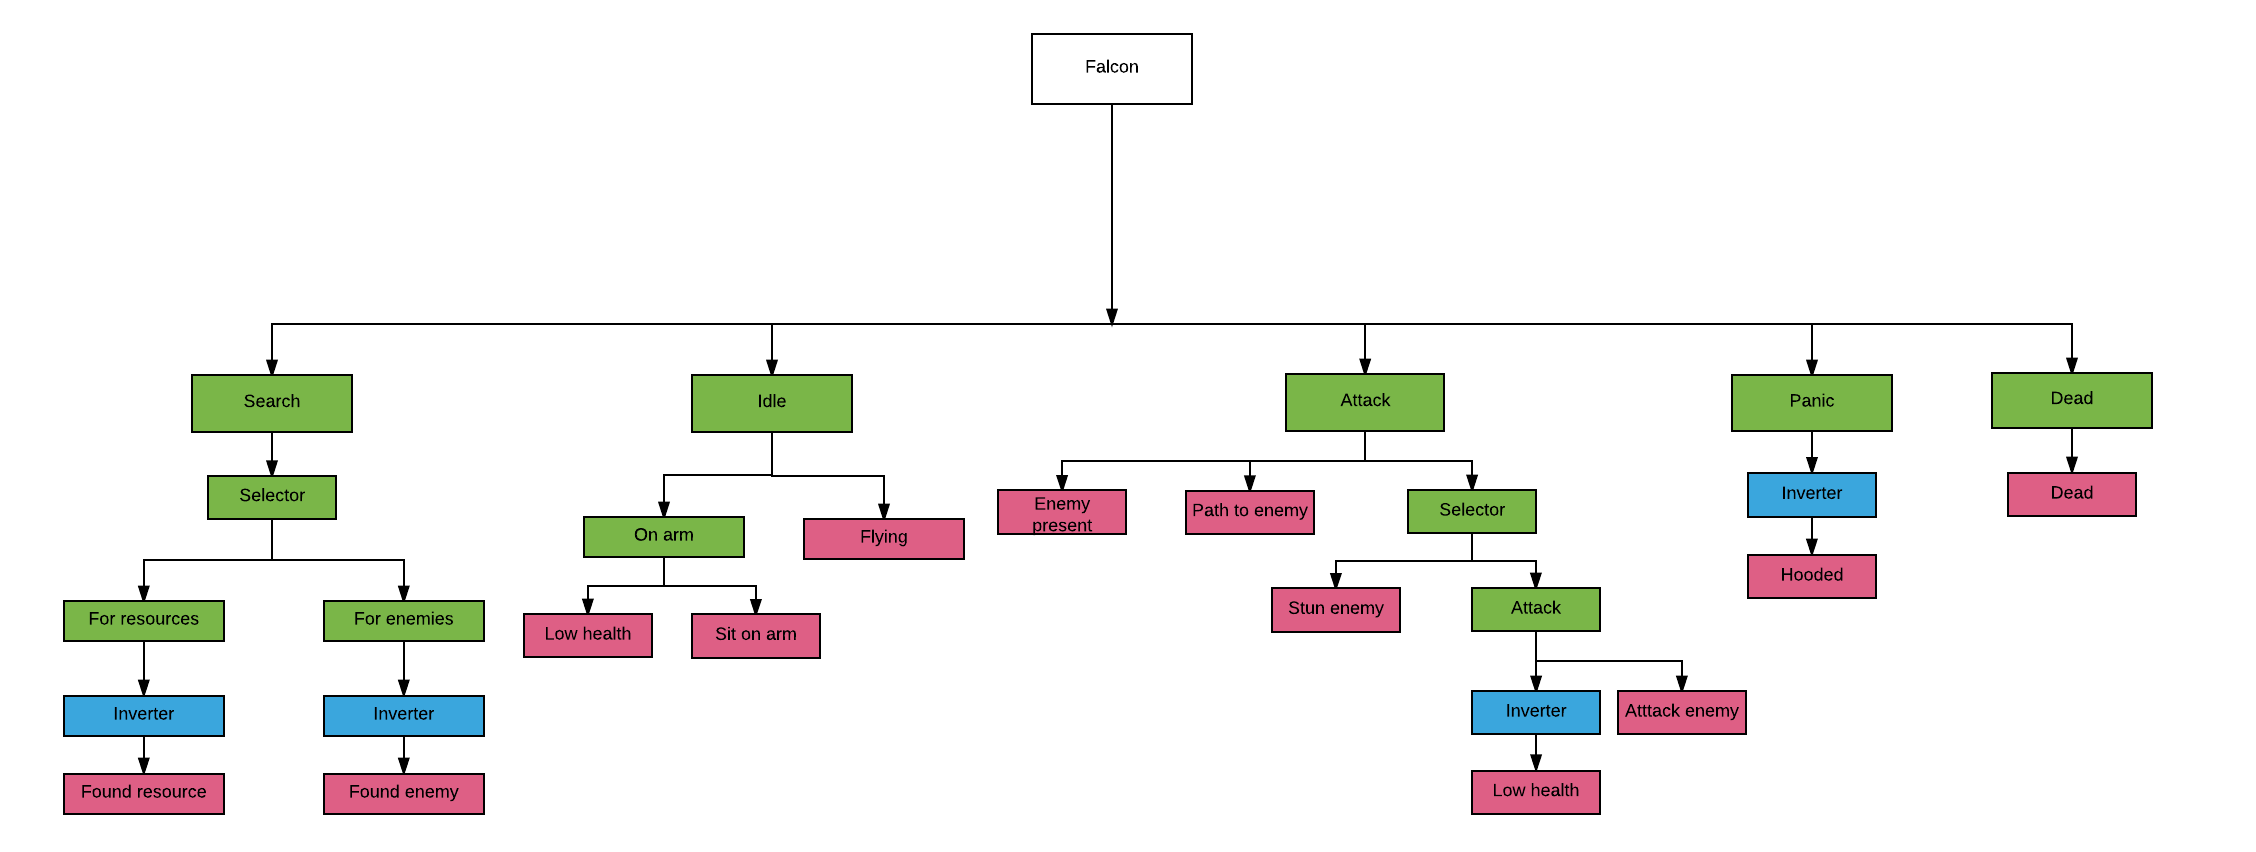
\includegraphics[width=1.2\linewidth]{behaviour_tree.png}
	\caption{ Behaviour tree being used on a falcon companion}
\end{figure} 

In figure 1 green represents sequence nodes, yellow is for selector nodes, blue for decorator and pink for leaf nodes.

The AI will search for useful objects for the player, search for enemies, attack/stun them and flee when injured.

When used with the navigable terrain generator the AI can use path finding to lead the player in the right direction. 

\section{Market Research}
Birds do not appear in games very often, they are mostly used as part of the environment that flies off when the player enter an area.
When researching companion AIs I found that they are often human \cite{DragonAge, LastOfUs, Bioshock}. There are also a number of features/behaviours that players say are required for a good AI companion. 

Two popular companions are Ellie from The Last of Us and Elizabeth from Bioshock Infinite. Both AIs aid the player by fetching helpful in game items, assisting in battles and leading the player towards the next goal in the game.
Guiding the player is a common behaviour in AI 


As VR games are relatively new games often use some sort of companion to guide the player \cite{RobinsonVR} .


companion AI system 
should be easy to adapt to other animals

- Navvi - ocarina of time
- wheatley portal



\section{Scope and Commercial Feasibility}
The scope of the component depends on the number of branches implemented. Once the nodes a working it's relatively easy to adapt and add branches.

There are numerous behaviour tree managing tools on the Unity Asset store where the price varies from being free to \pounds225. Most of the tools come with a GUI so mine would need to be significantly cheaper as it is a lot more difficult to use.
The Unity Asset store guidelines say that packages priced over \$50 are often the best selling ones. Also when looking at behaviour tree tools on the Asset store many of the best selling tools are above that price. This suggests that somewhere around \$50 would be a good price for my tool if I added a GUI to make it more accessible to users. As the target audience is indie game developers with little code experience or trying to make a quick prototype it would 
\bigskip

 A unique selling point is that most behaviour trees tools on the asset store are general tools not specific to companion AIs mine is specifically designed for companions.


Also using a platform such as the Unity Asset store will result in the store taking a cut of the money made from it 



\bibliographystyle{ieeetr}
\bibliography{comp230}
	
\end{document}
